\documentclass[11pt]{article}
\def\hidesolutions{}
%%%%%%%%%%% SET MARGINS
\setlength{\textheight}{20cm}
\setlength{\topmargin}{-0.5cm}
\setlength{\oddsidemargin}{+0cm}
\setlength{\textwidth}{16.3cm}
%\setlength{\parskip}{6pt}
\setlength{\parindent}{0pt}

%%%%%%%%%%% PACKAGES
\usepackage{amsmath}
\usepackage{amssymb}
\usepackage{amsfonts}
%\usepackage{a4wide}
\usepackage{graphicx}
\usepackage{color}
\usepackage[normalem]{ulem}
\usepackage{enumitem}
\usepackage{capt-of}
\usepackage{float}
\usepackage{amsmath}
\usepackage{listings}
\definecolor{mygreen}{RGB}{28,172,0} % color values Red, Green, Blue
\definecolor{mylilas}{RGB}{170,55,241}
\usepackage{empheq}
\usepackage[ruled]{algorithm2e}
\usepackage{mathrsfs}
\usepackage{datetime}
\usepackage{subcaption}

% TODO: combine the two package lists and reduce redundancies 
\usepackage{mathtools}
\usepackage{nicefrac}
\usepackage{hyperref}
\usepackage{url}
\usepackage{amsmath,amssymb,amsfonts}
\usepackage{a4wide}
\usepackage{graphicx}
\usepackage{color}
\usepackage[normalem]{ulem}
\usepackage{capt-of}
\usepackage{float}
\usepackage[ruled]{algorithm2e}
\usepackage{amsmath,amssymb,amsfonts}
\usepackage{a4wide}
\usepackage{graphicx}
\usepackage{color}
\usepackage[normalem]{ulem}
\usepackage{capt-of}
\usepackage{float}
\usepackage[ruled]{algorithm2e}
\usepackage{mathrsfs}







\newcommand{\Lc}[2]{{\color{blue} \sout{#1} } \textcolor{red}{#2}}
\newcommand{\La}[1]{\textcolor{red}{#1}}
\newcommand{\lh}{\mathscr{L}_h}
\newcommand{\cl}{\mathscr{L}}
\newcommand{\cf}{\mathscr{F}}
\newcommand{\dx}{dx}
% \newcommand{\d}{d}
\newcommand{\ltn}{\mathscr{l}^2}
\newcommand{\bbR}{\mathbb{R}}
\newcommand{\Rset}{\mathbb{R}}
\newcommand{\Nset}{\mathbb{N}}
\newcommand{\scL}{\mathcal{L}}
\newcommand{\xx}{\mathbf{x}}
\newcommand{\norm}[1]{\|{#1}\|}
\newcommand{\yy}{\mathbf{y}}
\newcommand{\at}[1]{\big|_{#1}}
\renewcommand{\div}{\mathrm{div}}
\newcommand{\divergence}{\mathrm{div}}
\newcommand{\cp}[1]{\textcolor{blue}{#1}}

\newcommand{\FF}{\texttt{FreeFem++ }}
\newcommand{\FFns}{\texttt{FreeFem++}}
\newcommand{\FFfull}{\texttt{FreeFem++-x11}}
\newcommand{\cmd}[1]{ \medskip \noindent \texttt{#1} \medskip}
\newcommand{\incmd}[1]{\texttt{#1}}
\newcommand{\shrinkitems}{\addtolength{\itemsep}{-0.5\baselineskip}}
\newcommand{\mtt}[1]{\mathtt{#1}}
\newcommand{\ML}{\texttt{Matlab }}

\newcommand{\bb}{\mathbf{b}}
\newcommand{\nn}{\mathbf{n}}
\newcommand{\vecA}{\vec{A}}
\newcommand{\vecB}{\vec{B}}


\newcommand{\frakF}{\mathfrak{F}}


\newcommand{\mesh}{\mathcal{T}_h}
\newcommand{\refel}{\widehat{K}}
\newcommand{\ver}{\mathbf{a}}
\newcommand{\refver}{\widehat{\mathbf{a}}}
\newcommand{\grad}{\nabla}
\newcommand{\refgrad}{\widehat{\nabla}}
\newcommand{\refu}{\widehat{u}}
\newcommand{\refbasis}{\widehat{\varphi}}
\newcommand{\refxx}{\widehat{\xx}}
\newcommand{\refx}{\widehat{x}}
\newcommand{\refy}{\widehat{y}}
\newcommand{\refrho}{\widehat{\rho}}
\newcommand{\refh}{\widehat{h}}

\makeatletter
\newcommand\suchthat{%
 \@ifstar
  {\mathrel{}\middle|\mathrel{}}
  {\mid}%
}
\makeatother





% For typesetting Python code
\newcommand{\matlab}{{\sc Matlab}\xspace}
\usepackage{listings}
\lstloadlanguages{Python}
\lstloadlanguages{csh}%
\definecolor{MyDarkGreen}{rgb}{0.0,0.4,0.0}
\definecolor{purple}{rgb}{0.58,0,0.82}
\lstset{language=Python,                    % Use Python
	%frame=single,                          % Single frame around code
	basicstyle=\ttfamily\footnotesize\color{black},
	keywordstyle=[1]\color{blue}\bf,        % Python functions bold and blue
	keywordstyle=[2]\color{purple},         % Python function arguments purple
	keywordstyle=[3]\color{red}\underbar,   % User functions underlined and blue
	commentstyle=\usefont{T1}{pcr}{m}{sl}\color{MyDarkGreen}\small,
	stringstyle=\color{purple},
	showstringspaces=false,                 % Don't put marks in string spaces
	tabsize=3,                              % 5 spaces per tab
	morekeywords={xlim,ylim,var,alpha,factorial,poissrnd,normpdf,normcdf},
	morecomment=[l][\color{blue}]{...},
	breaklines=true,
	breakatwhitespace=true,
	emptylines=1,
	mathescape=true,
	xleftmargin=0ex,
	emphstyle=\bfseries\color{red}
}





%%%%%%%%%%% MACROS NAMES
\newcommand{\lecturername}{Martin Licht}
% \newcommand{\assistantnamea}{Jochen Hinz}
% \newcommand{\assistantnameb}{Ivan Bioli}
\newcommand{\semestername}{Winter Semester 2024}
\newcommand{\lecturename}{Analysis III - 203(d)}
\DeclarePairedDelimiter\floor{\lfloor}{\rfloor}

%%%%%%%%%%% HEADER
\newdateformat{yeardate}{\THEYEAR}
\newcommand{\exsheet}[3] % input is the number of the session and the day TODO What's that
{\clearpage

	\begin{center}
		{\Large \textbf{\lecturename}}\\[2ex]
		\semestername
	\end{center}

	% \vspace{2ex}
	% \lecturername

	\vspace{2ex}
	{\Large Session #1: #3\,#2, \yeardate\today}
	%\hfill
	%{\Large EPF Lausanne}

	\hrulefill
}





\usepackage{comment}

\newtheorem{exercise}{Exercise}
\newtheorem{solutionenv}{Solution}

\newboolean{hide_solution}
\ifx\hidesolutions\undefined
\newenvironment{solution}{\begin{solutionenv}}{\end{solutionenv}}
\setboolean{hide_solution}{false}
\else
\excludecomment{solution}
\setboolean{hide_solution}{true}
\fi

\newcommand{\ifnotsolution}[1]{\ifthenelse{\boolean{hide_solution}}{#1}{}}
\newcommand{\ifsolution}[1]{\ifthenelse{\boolean{hide_solution}}{}{#1}}


\usepackage{tikz}
\usepackage{pgfplots}





\allowdisplaybreaks

\begin{document}
\exsheet{8}{7}{November} % parameters are the number of the session and the day



\begin{exercise}
    Consider the following functions with period $T$:
    \begin{itemize}
        \item A function $f$ with period $T = 1$ such that 
        \begin{align*}
            f(x) = 
            \left\{\begin{array}{ll}
                1 & \text{if } 0 \leq x < 0.5 \\
                0 & \text{if } 0.5 \leq x \leq 1
            \end{array}\right.
        \end{align*}
        \item A function $g$ with period $T = 2\pi$ such that 
        \begin{align*}
            g(x) = 
            \left\{\begin{array}{ll}
                x & \text{if } 0 \leq x < \pi \\
                2\pi - x & \text{if } \pi \leq x \leq 2\pi
            \end{array}\right.
        \end{align*}
        \item A function $h$ with period $T = 1$ such that 
        \begin{align*}
            h(x) = -x \text{ if } 0 \leq x < 1.
        \end{align*}
    \end{itemize}
    Find the Fourier coefficients of the Fourier series of these functions. 
    \textit{You can modify the functions seen in the lecture to get the coefficients.}
\end{exercise}


\begin{exercise}
    Explicitly write down the coefficients $a_n$ and $b_n$ and the periods of the following Fourier series:
    \begin{align*}
        f(x) &= \sum_{n=1}^{\infty} \frac{1}{(2n+1)^2}\sin(2\pi (2n+1) x),
        \\
        g(x) &= \sum_{n=1}^{\infty} \frac{(-1)^n}{(2n-1)^3}\cos(2\pi (2n-1) x),
        \\
        h(x) &= \frac \pi 3 + \sum_{n=1}^{\infty} \frac{(-1)^{n+1}}{n^2}\cos(\pi n x),
        .
    \end{align*}
    Determine the Fourier coefficients of the derivatives of those functions. 
\end{exercise}
\begin{solution}     
    % n = 3, 5, 7, ... T=1, 
    % n = 1, 3, 5, ... T=1, 
\end{solution}


\begin{exercise}[Green's theorem]
    Consider the following closed curve $C$:
    \begin{center}
    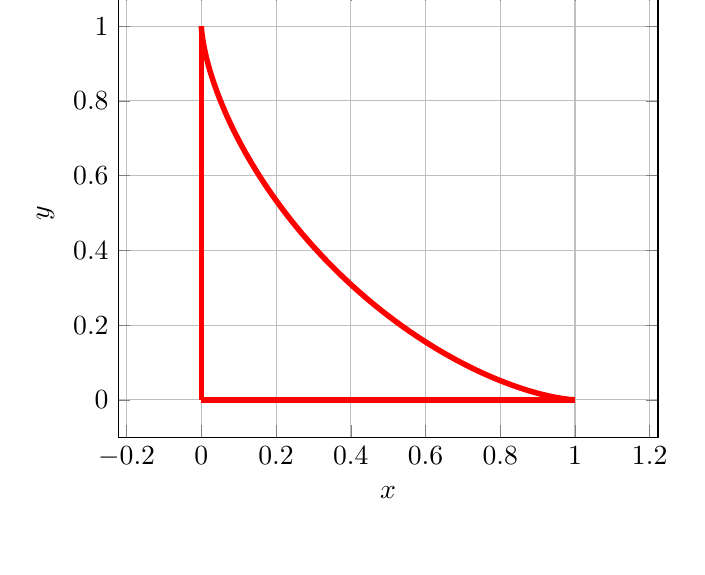
\begin{tikzpicture}
        \begin{axis}[
            xlabel={$x$},
            ylabel={$y$},
            axis equal,
            grid=major,
            domain=0:1,
            samples=200,
        ]
        \addplot+[mark=none,color=red, line width=2pt] ({sin(deg(x*pi/2))^3}, {cos(deg(x*pi/2))^3});
        \addplot+[mark=none,color=red, line width=2pt] ({0}, {x});
        \addplot+[mark=none,color=red, line width=2pt] ({x}, {0});
        \end{axis}
    \end{tikzpicture}
    \end{center}
    The curved part of the curve can be parameterized by 
    \begin{align*}
        \gamma : \left[0,\frac{\pi}{2}\right] \to \bbR^2, \quad t \mapsto \left( \cos^3(t), \sin^3(t) \right).
    \end{align*}
    \begin{itemize}
        \item Find parameterizations of the other two curves.
        \item With the $\vec F(x_1,x_2) = (x_2,-x_1)$ compute the curve integral 
        \[ \oint_C \vec F dl \]
        \item Use Green's theorem to explain how to compute the size of the area enclosed by the curve $C$.
    \end{itemize}
\end{exercise}
\begin{solution}     
\end{solution}


\begin{exercise}[Stokes's theorem]
    We have a vector field 
    \begin{align*}
        \vec F( x_1, x_2, x_3 ) = \left( x_1 x_2, x_2 x_3, x_1 x_3 \right)
    \end{align*}
    and a surface 
    \begin{align*}
        S := \left\{ (x_1,x_2,x_3) \in \bbR^{3} \suchthat* x_1^2 + x_2^2 + x_3^2 = 1, \; x_2 \geq 0, x_3 \geq 0 \right\} 
    \end{align*}
    \begin{itemize}
        \item Find parameterizations of the surface $S$ and a parameterization of its boundary curve $C$.
        \item Use Stokes' theorem to compute the integral 
        \begin{align*}
            \iint_{S} \vec F \;d\sigma.
        \end{align*}
    \end{itemize}
\end{exercise}
\begin{solution}     
\end{solution}













% 
% 
% 
% \begin{exercise}
%     \textit{This is for fun and entertainment only.}
%     Compute 
%     \[
%         \sqrt{ 500 \cdot 501 \cdot 502 \cdot 503 + 1 }
%     \]
%     without using a calculator.
% \end{exercise}
% \begin{solution}
%     Inside the square root, we find 
%     \begin{align*}
%         &
%         500 \cdot 501 \cdot 502 \cdot 503 + 1
%         \\&=
%         500 \cdot (500+1) \cdot (500+2) \cdot (500+3) + 1
%         \\&=
%         500^4 + 6 \cdot 500^3 + ( 2 + 3 + 6 ) \cdot 500^2 + 6 \cdot 500 + 1
%         \\&=
%         500^4 + 6 \cdot 500^3 + 11 \cdot 500^2 + 6 \cdot 500 + 1
%         .
%     \end{align*}
%     A sharp look reveals that this equals 
%     \begin{align*}
%         &
%         500^4 + 6 \cdot 500^3 + 11 \cdot 500^2 + 6 \cdot 500 + 1
%         =
%         ( 500^2 + 3 \cdot 500 + 1 )^2
%         .
%     \end{align*}
%     Therefore,
%     \[
%         \sqrt{ 500 \cdot 501 \cdot 502 \cdot 503 + 1 } = 500^2 + 3 \cdot 500 + 1 = 250000 + 1500 + 1
%     \]
%     The total result is $251501$. Which happens to be a prime number.
% \end{solution}

\end{document}
